\section{Show me music}
Capbussa't en un munt de temes que mostren les complexes interrelacions de la melodia, l'harmonia i les matemàtiques. Cada animació s'assembla a certes peces o patrons des d'alguns punts de vista matemàtics. Alguns aspectes de simetria, tant en l'espai com en el temps, ajuden a entendre idees musicals.

\begin{figure}[!h]
\centering
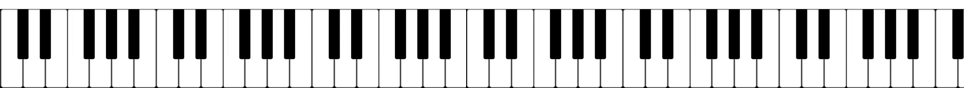
\includegraphics[width=\textwidth]{ShowMeMusic_1}
\end{figure}

\subsection{Spiral Tone Space}
Les tecles d'un piano formen un patró força regular. Entre cada grup de set lletres blanques el patró de tecles blanques i negres es repeteix. Si toques el piano i decideixes tocar vuit tecles blanques més a la dreta, la música sonarà gairebé igual... només que serà una octava més alta. Una bona manera d'expressar aquest fet de forma matemàtica és col·locar els tons en una espiral de manera que cada volta completa es correspon exactament amb una octava.

\begin{figure}[h]
\centering
\begin{subfigure}{0.45\textwidth}
\centering
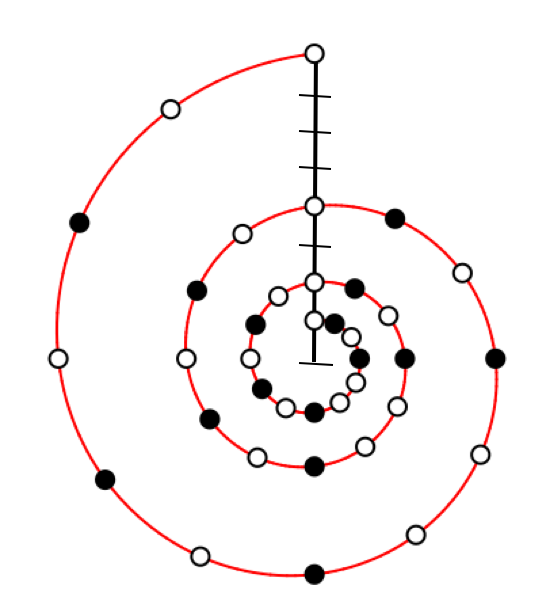
\includegraphics[height=4cm]{ShowMeMusic_2}
\end{subfigure}
\begin{subfigure}{0.45\textwidth}
\centering
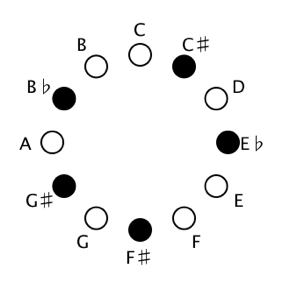
\includegraphics[height=4cm]{ShowMeMusic_3}
\end{subfigure}
\end{figure}


\paragraph{La Música:} El concepte d'una octava és pràcticament omnipresent a la música. Fins i tot entre cultures diferents. Tocar una cançó una octava més amunt significa essencialment duplicar totes les freqüències. Això està estretament relacionat amb les sèries de sobretons. Un piano normalment té una mica més de 7 octaves. En canvi, el rang vocàlic humà és del voltant de 2 octaves.


\paragraph{Les Mates:} La figura de sobre il·lustra una seqüència de tres octaves en forma d'espiral logarítmica. Els tons greus estan situats més a prop del centre de l'espiral. Comença amb un Do i es mou en espiral en el sentit horari cap a notes més i més altes. Per poder-les seguir, s'ha utilitzat l'ordre de les tecles blanques i negres del piano. L'escala de l'espiral s'ha triat de manera que a cada volta completa es correspon a una octava i la distància de qualsevol punt fins al centre és proporcional a la seva freqüència. D'aquesta manera, al voltant del raig negre vertical, pots veure quatre Do diferents. Cadascun dels dotze raigs es correspon a cadascuna de les notes del nostre sistema de dotze tons. En funció del context, és comú i raonable no distingir entre notes igual de diferents octaves, això ens porta a l'anomenat espai tonal circular.

\paragraph{El Mòdul:} El mòdul visualitza els tons de cançons molt conegudes a l'espai tonal en espiral. Els paràmetres d'escala de l'espiral es trien de forma lleugerament diferent si cal veure més o menys octaves. Les notes predominants (a l'espai tonal circular) es detecten automàticament i s'assenyala adequadament la classe corresponent. Amb això pots seguir les notes dominants d'una cançó. Gaudeix escoltant i veient la música! Fins i tot cançons molt conegudes poden revelar patrons ocults i fer la composició més transparent.

\subsection{Space of Three-Note Chords}
A vegades apareixen estructures sorprenents si un estudia objectes des d'un punt de vista en què no només té en compte un objecte sinó diversos i les seves relacions. Per exemple, considerar totes les possibilitats per tocar un acord de tres notes dóna lloc a un objecte geomètric sorprenentment ric. Per això, ignorarem la informació de l'octava, de manera que tots els Do es tracten igual. La fotografia següent mostra aquest espai. Cada punt correspon a un possible acord. Resulta que aquest espai forma un prisma triangular que conté tots els 364 possibles acords. Cada punt correspon a tres notes . Els tres costats verticals corresponen a situacions on les tres notes són idèntiques. L'eix central de punts blancs correspon a acords de terceres encadenades. En aquest cas: Do - Mi - Sol$\sharp$


\begin{figure}[h]
\centering
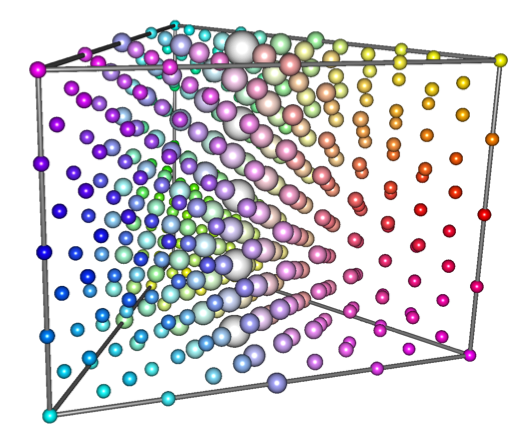
\includegraphics[width=0.6\textwidth]{ShowMeMusic_4}
\end{figure}

Els acords que es troben a prop d'altres en aquest espai es diferencien per un semitò. Fer petits canvis d'un acord a l'altre (amb moviments de semitò) significa voltar per l'estructura. Si fixem dues notes d'un acord i canviem l'altra en salts de semitò obtenim un camí lineal dins del prisma. Els costats quadrangulars actuen com parets o miralls on els camins reboten. Els costats superior i inferior estan també relacionats. Si intentes creuar el costat superior, aconsegueixes arribar a la part inferior, i viceversa.

\begin{wrapfigure}[18]{l}{0.35\textwidth}
\centering
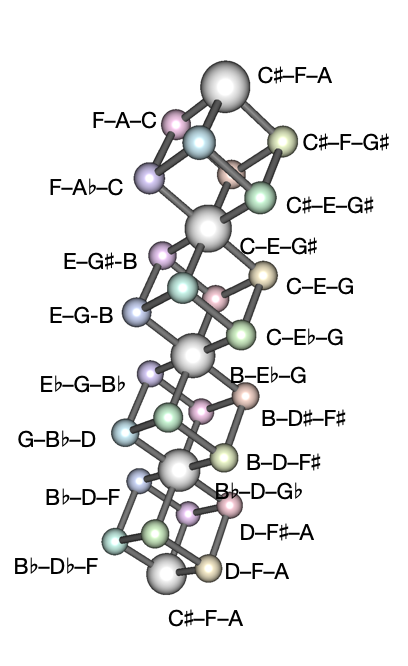
\includegraphics[width=0.34\textwidth]{ShowMeMusic_6}
\end{wrapfigure}
\paragraph{La Música:}  Aquesta estructura 3D codifica un munt de teoria musical clàssica. Per exemple, a una distància 1 de l'eix central pots trobar tots els acords majors i menors. A la fotografia s'etiqueten diversos acords. Les progressions clàssiques d'acords sovint es corresponen a passeigs per aquesta estructura.

\paragraph{Les Mates}: Aquesta imatge té moltes relacions profundes amb la teoria de la simetria. El fet que les cares quadrangulars actuïn com a miralls i que la superior i la inferior s'identifiquin fa que el prisma sigui fonamentalment una cel·la d'objectes tridimensionals en el qual infinits d'aquests prismes omplen tot l'espai. Just com un fons d'escriptori tridimensional simètric.  Considerar l'espai d'acords d'una manera tan genèrica és un  camp d'estudi relativament nou i que principalment dirigeix el professor Dimitri Tymoczko a Princeton.\\


\paragraph{El Mòdul:} El mòdul et permet navegar l'espai d'acords mencionat. La bola vermella indica la posició actual. Es toca un arpegi aleatori de l'acord seleccionat. Mou-te entre els acords, escolta'ls i crea les teves pròpies progressions musicals!

\begin{figure}[h]
\centering
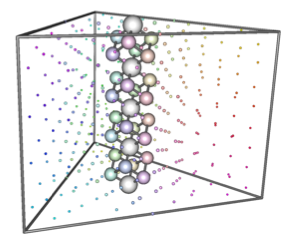
\includegraphics[width=0.5\textwidth]{ShowMeMusic_5}
\end{figure}


\subsection{Pachelbels Canon in D and Pachelballs}
El Cànon en Re de Pachelbel és, potser, una de les obres clàssiques més conegudes. Tot i que es va compondre l'any 1609 (segurament abans que l'obra de Back) sona sorprenentment fresc i modern. Segueix un esquema d'acords impressionant que fins i tot en l'actualitat forma part de la base de cançons molt conegudes de Pop, Folk, Country i Jazz com ara Skater Boy d'April Lavigne, No Woman No Cry de Bob Marley o Let it be dels Beatles.

\paragraph{Les Mates:} Un cànon és repetició i la repetició és simetria. En certa manera, un cànon és simetria en el temps. Es repeteix el mateix patró cada vegada que passa certa estona. De fet, el Cànon de Pachelbel és lleugerament diferent a la resta de cànons, ja que el patró musical de cada veu no es repeteix passada una estona.

\paragraph{La Música:} EL fet que les veus individuals no es repeteixin permeten a Pachelbel crear una progressió de densitat al cànon (a diferència d'altres). Pachelbel compon amb molts girs complicats tant rítmicament com melòdicament. A més a més, els patrons que fa la veu principal acaben convertint-se en l'acompanyament al cap d'uns moments.

\paragraph{El  Mòdul:} Dos dels nostres mòduls es basen en el Cànon de Pachelbel. Un d'ells visualitza la peça sencera i emfatitza el fet que les tres veus toquen exactament la mateixa partitura amb un desplaçament temporal, l'altre (Pachelballs) és un joc. Basant-te en els patrons d'acords de Pachelbel pots crear fragments molt agradables.

\begin{figure}[t]
\centering
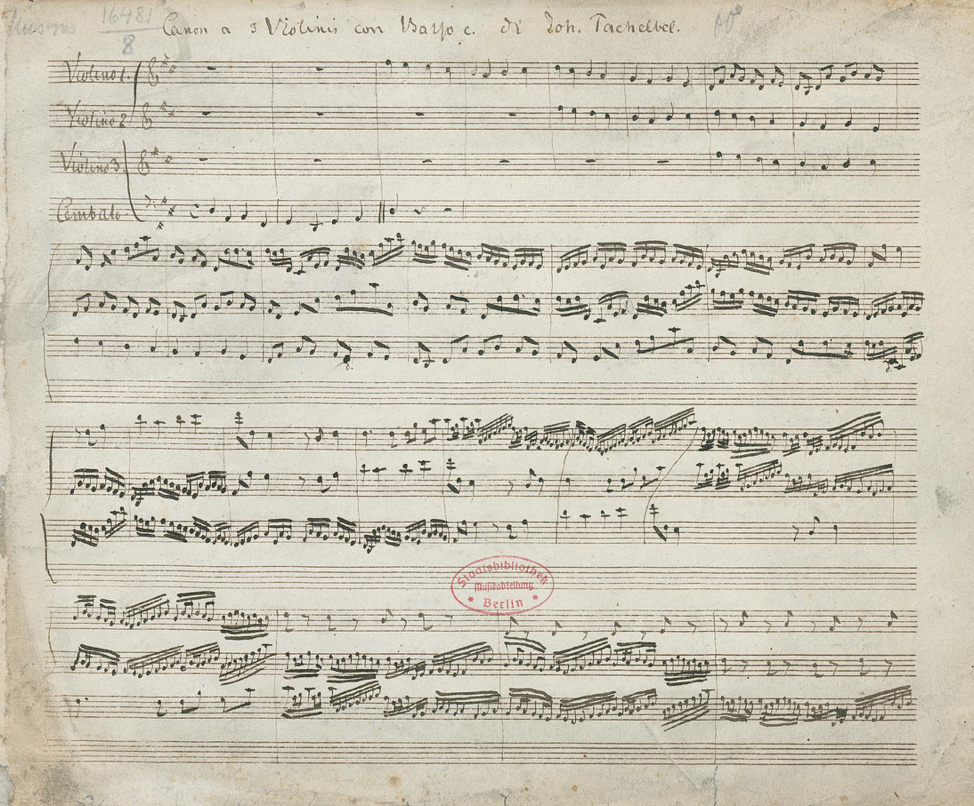
\includegraphics[width=0.7\textwidth]{ShowMeMusic_7}
\end{figure}


\subsection{Mozart's Musical Dice Game}
Alguns anys després de la mort de Mozart es va publicar un dau musical. Aquest se li atribueix, ja que molt probablement era la seva invenció. En termes moderns, en podríem dir un generador de música aleatori. El joc permet la creació d'un minuet que sona bé i que el més possible és que no s'hagi tocat mai. Per això, Mozart presenta una partitura amb compassos numerats. Amb la partitura hi ha una taula per cada compàs amb possibles compassos que es poden utilitzar per omplir els espais buits. El compàs que s'utilitza en cada cas es determina tirant dos daus, sumant-ne el resultat i seleccionant la fila corresponent. Sorprenentment, l'estil de cada vals que es crea d'aquesta manera recorda molt a l'estil de Mozart.


\paragraph{La Música:} Com ho van fer? A primera vista, molta gent es va sorprendre per la música creada amb aquest procediment. Si hi donem una ullada més profunda, ja no resulta tan sorprenent. El contingut principal conceptualment es determina més aviat per la progressió harmònica que no per la melodia concreta de la cançó. Per una harmonia donada hi ha moltes maneres melòdiques d'expressar la mateixa idea. El que va fer Mozart és simplement oferir 11 possibilitats ``equivalents'' per cada compàs. És com substituir la frase ``L'ordinador està espatllat'' amb ``L'ordinador no funciona''. Per aquesta raó, els minuets creats amb aquest joc sonen més o menys igual.


\begin{wrapfigure}[22]{r}{0.4\textwidth}
\centering
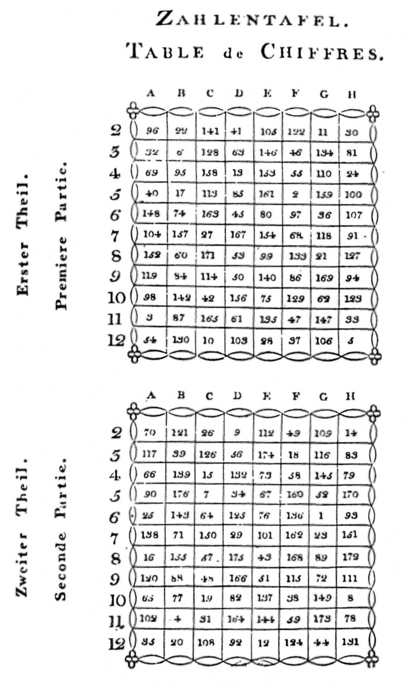
\includegraphics[width=0.4\textwidth]{ShowMeMusic_8}
\end{wrapfigure}

\paragraph{Les Mates:} La primera pregunta i potser la més obvia és quantes possibles cançons es poden crear amb aquest joc? El vals té dues parts. Cadascuna té vuit compassos. Per cada compàs hi ha un total d'onze possibilitats. Amb una mica de combinatòria descobrim que hi ha l'astronòmic total de $11^{16} = 45 949 729 863 572 161$ possibilitats. Escoltar-les totes requeriria al voltant de 60 bilions d'anys. Creu-me, ja t'hauries avorrit.

També hi ha un subtil punt matemàtic en aquest joc. La distribució de compassos no serà una distribució igual. Com que cada compàs es tria amb la suma dels resultats de dos daus hi ha una tendència cap als nombres centrals. Hi ha un total de $6\times 6=36$ possibles resultats de les tirades dels dos daus. Només una d'aquestes, 1+1=2, creen el número 2, però n'hi ha sis que creen el número 7 = 1+6 = 2+5 = 3+4 = 4+3 = 5+2 = 6+1.

\paragraph{El Mòdul:} Si vols la teva peça individual de Mozart que, a més a més, no s'ha sentit mai, només has de prémer el botó i gaudir!

\subsection{Shepard Tone}

\begin{wrapfigure}[39]{l}{0.25\textwidth}
\centering
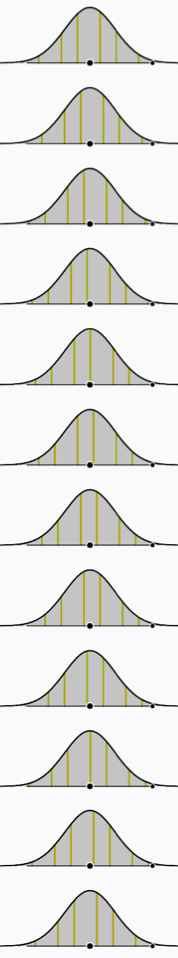
\includegraphics[height=0.9\textheight]{ShowMeMusic_9}
\end{wrapfigure}

La percepció és una cosa estranya. A vegades sentim o veiem coses que no hi són realment. Hi ha una il·lusió acústica que crea l'efecte d'un to que sempre puja o sempre baixa. El concepte és similar al de les escales d'Escher, que sembla que pugin amb cada pas, però realment només es mouen en cercles.

Aquesta il·lusió es crea de la següent manera: es defineix una finestra de freqüència, idealment amb límits suaus. Això es pot fer, per exemple, amb una campana de Gauss. En aquesta finestra tots els sobretons d'un cert espectre i que pertanyen al to es toquen. L'amplitud dels diferents tons parcials es determina segons la finestra. Ara l'espectre està desplaçat cap a la finestra. Mentre els sobretons greus s'esvaeixen gradualment, noves notes més agudes entren a la finestra. Mirant la mitjana, la freqüència es manté igual. Tot i això sona com un to descendent. Aquest edicte s'anomena To de Shepard

\paragraph{La Música:} És extremadament difícil tocar un To de Shepard convincent en un instrument clàssic i no electrònic. Requereix un control increïble sobre la intensitat de les notes tocades. Tanmateix, es va utilitzar per compositors moderns en diverses peces: la banda sonora de Hans Zimmer de la pel·lícula Dunkerque, el final de Echoes de Pink Floyd i fins i tot la banda sonora del joc Super Mario quan el protagonista corre per una escala sense fi.

\paragraph{Les Mates:}Crear un to de Shepard requereix precisió. Els tons han d'entrar i  sortir de l'espectre gairebé sense que ens n'adonem. Una bona manera de modelar-ho és utilitzant la campana de la distribució Gaussiana per controlar la intensitat dels sons que es toquen. Amb això, fins i tot un rang petit de freqüències fan un bon efecte. No obstant això, com més extens i més ric sigui l'espectre escollit més convincent és l'efecte. La fotografia mostra el sonograma d'un To de Shepard.

\paragraph{El Mòdul:}Amb el nostre mòdul pots controlar diversos paràmetres del To de Shepard controlant la forma i posició de la corba Gaussiana involucrada. Explora la llibertat que hi ha a l'hora de crear aquesta il·lusió acústica.

\begin{figure}[h]
\centering
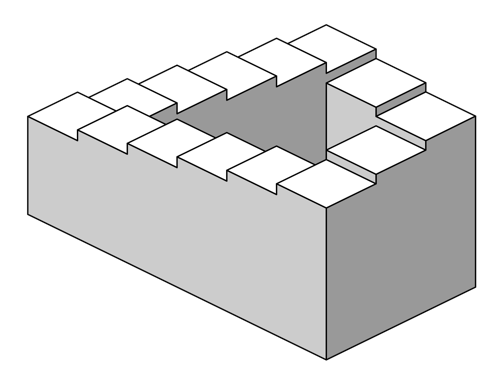
\includegraphics[width=0.5\textwidth]{ShowMeMusic_10}
\end{figure}
\strut
\vspace{6em}

\begin{sectcredits}
\item[Autor del mòdul:] Jürgen Richter-Gebert (Technical University of Munich).

\item[Agraïments:] Patrick Wilson i Aaron Montag (sistema de so) Basat en CindyJS.org

\item[Text:] Jürgen Richter-Gebert (TU Munich).
\end{sectcredits}
